
\documentclass[a4paper, 12pt, oneside]{article}
\usepackage[utf8]{inputenc}
\usepackage{graphicx}
\usepackage{tabularx}
\usepackage[export]{adjustbox}
\usepackage{paralist}
\usepackage{wrapfig}
\usepackage{float}
\usepackage{geometry}
\usepackage{subcaption}
\usepackage[singlelinecheck=false]{caption}
\begin{document}

\begin{titlepage} % Suppresses headers and footers on the title page

	\centering % Centre everything on the title page
	
	\scshape % Use small caps for all text on the title page
	
	\vspace*{\baselineskip} % White space at the top of the page
	
	%------------------------------------------------
	%	Title
	%------------------------------------------------
	
	\rule{\textwidth}{1.6pt}\vspace*{-\baselineskip}\vspace*{2pt} % Thick horizontal rule
	\rule{\textwidth}{0.4pt} % Thin horizontal rule
	
	\vspace{0.75\baselineskip} % Whitespace above the title
	
	{\LARGE Consultant Tracker\\Testing Policy} % Title
	
	\vspace{0.75\baselineskip} % Whitespace below the title
	
	\rule{\textwidth}{0.4pt}\vspace*{-\baselineskip}\vspace{3.2pt} % Thin horizontal rule
	\rule{\textwidth}{1.6pt} % Thick horizontal rule
	
	\vspace{2\baselineskip} % Whitespace after the title block
	
	
	%------------------------------------------------
	%	Editor(s)
	%------------------------------------------------
	
	Edited By
	
	\vspace{0.5\baselineskip} % Whitespace before the editors
	
	{\scshape\Large Sibekezelo Mamba 16095414 \\ Johan de Waal 16155140 \\ Stephen Munro 16024479\\ Hulisani Mudimeli 16073364 \\ Ngonidzashe Mujuru 16285256  \\ Tatenda Mafunga 16094965\\} % Editor list
	
	\vspace{0.5\baselineskip} % Whitespace below the editor list
	
	\textit{University of Pretoria \\2018} % Editor affiliation
	
	\vfill % Whitespace between editor names and publisher logo
	
\end{titlepage}

\newpage
\tableofcontents
\newpage


\pagenumbering{arabic}


\pagebreak



\section{Introduction}



Travis CI (Continuous Integration) improves development process by automatically building and testing code modifications which in turn provides instant response or feedback on the status of the modification.
\\\\
Travis CI is linked with our GitHub repository that contains our project source code. Travis was chosen because it makes use of continuous integration which is a development practice that joins small code alterations or modifications regularly instead of merging a large change when development cycle is completed.




\section{Overview}

Travis CI use its own system to perform tests. The automation of executions does not depend on the speed or performance of an individual’s machine. Results of the tests are sent via email and shown in the Travis job status section.


\section{Variances}

Multiple conditions and events were detected during the test. This includes the condition of having to delete something that never existed. Travis helped integrate the test steps to avoid that risky condition from happening. The test cases below will elaborate further on how this was solved. \\\\Most test cases were successful only when the tomcat server and the database server where running, otherwise, it would produce an error because of failure to communicate with the database.



\section{Assessment}
Java was used for back-end by the implementation of servlets that exchanges data with the front-end of our system. Individual units of source code of the system, associated with usage methods, data control and operating procedures will be tested using Unit Testing to ensure that the code works as it is intended to.
\pagebreak
Testing Framework: Travis Continuous Integration\\
Module Tested: Java Test Files that in turn tests the servlets\\
Test Cases:\\
\hspace*{10mm}a)	Creating Projects\\
\hspace*{10mm}b)	Adding Consultants\\
\hspace*{10mm}c)	Removing Consultants\\
\hspace*{10mm}d)	Deleting Projects\\

\section{Results}
The following results shows the executed test cases’ output and shows that all test cases have passed the test. All test cases used separate java files to test the individual parts of the system.

\subsection{Test Case 1: Creating a project}

After the execution of test case one, the database was populated with an extra Project called Dummy-Project. This test case was successful only when the tomcat server and the database server where running.

\begin{figure}[!htb]

\centering

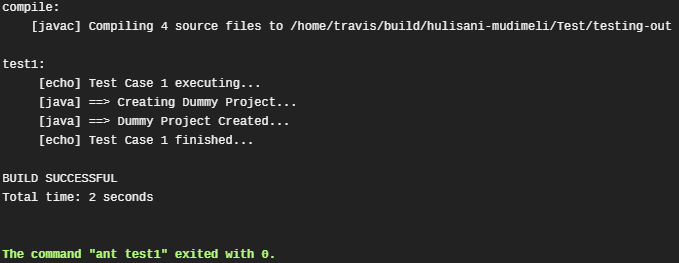
\includegraphics[width=\linewidth]{images/test1.png}

\caption{Creating Project}

\label{fig:sfig1}

\end{figure}


\subsection{Test Case 2: Adding Consultants to a project}

Test Case 2 requires Test Case 1 to be successful so that consultants can be added to the desired Project. Upon execution test case 2, Dummy-Project had a consultant added to it. This test case was successful only when the tomcat server and the database server where running.

\begin{figure}[!htb]

\centering

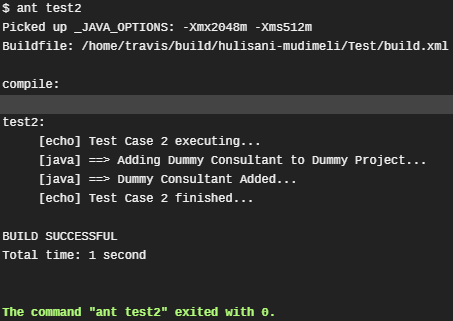
\includegraphics[width=10cm]{images/test2.png}

\caption{Add Consultant to Project}

\label{fig:sfig1}

\end{figure}


\subsection{Test Case 3: Removing a consultant}

Test Case 3 requires Test Case 2 to be successful so that a consultant can be removed from the Dummy Project. Upon execution test case 3, Dummy-Project had the dummy consultant removed from it. This test case was successful only when the tomcat server and the database server where running.

\begin{figure}[!htb]

  \centering

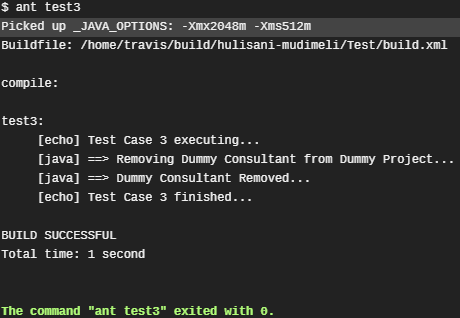
\includegraphics[width=10cm]{images/test3.png}

  \caption{Remove Consultant from Project}

  \label{fig:sfig1}

\end{figure}

\pagebreak
\subsection{Test Case 4: Deleting a Project}
Test Case 4 requires Test Case 1 to be successful so that the created dummy project exists for removal. Upon execution test case 4, Dummy-Project was removed from the database. This test case was successful only when the tomcat server and the database server where running.

\begin{figure}[!htb]

  \centering

  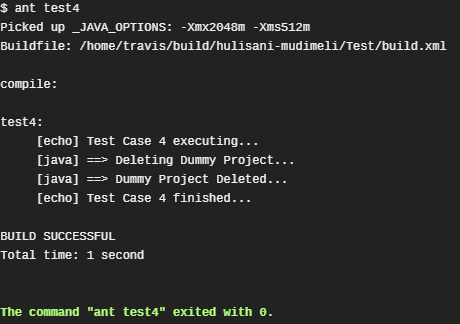
\includegraphics[width=10cm]{images/test4.png}

  \caption{Delete Project}

  \label{fig:sfig1}

\end{figure}

\pagebreak
\section{Evaluation}

All four test cases for Consultant Tracking went through extensive automated testing by the help of the testing tool, Travis CI. After the execution of all this four test cases, errors would have occurred only when trying to remove a consultant that was never created and when trying to delete a project that never existed. But our automation process was programmed to follow the no erroneous steps such that no consultant or project is removed without their existence. Therefore, no errors where produced by our automated testing

\section{Summary of Activities}

The automated testing execution only took, 32 seconds to run all the configurations that have been specified in the .travis.yml file.
\begin{figure}[!htb]

  \centering

   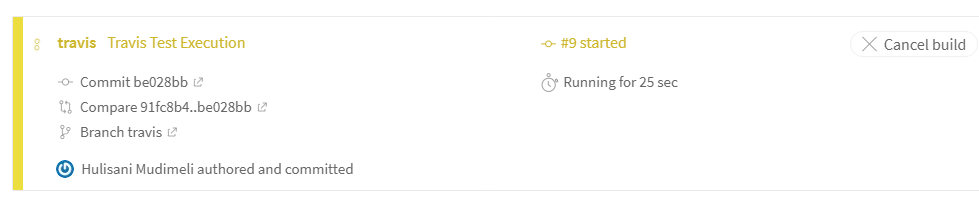
\includegraphics[width=\linewidth]{images/Capture.png}

\caption{Testing in progress}

 \label{fig:sfig1}

\end{figure}

\begin{figure}[h]

  \centering

   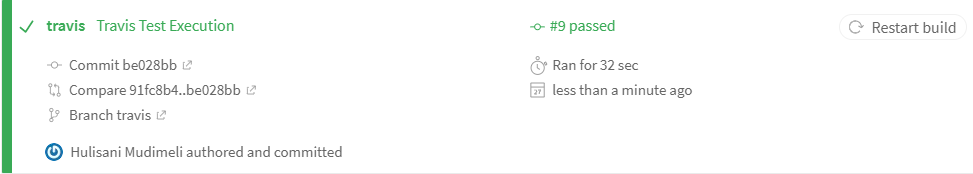
\includegraphics[width=\linewidth]{images/Capture3.png}

\caption{Testing completed}

 \label{fig:sfig1}

\end{figure}
\end{document}
